\cleardoublepage
\section{Umsetzung} \thispagestyle{nomarkstyle}
In diesem Kapitel werden die wichtigsten Aspekte der Umsetzung der in \cref{specification} beschriebenen Spezifikation behandelt, sowie exemplarisch einige Implementierungsdetails vorgestellt.
 
\subsection{Initiales Aufsetzen der Anwendung}
Bevor mit der Entwicklung begonnen werden kann, müssen die grundlegenden Bausteine der Anwendung angelegt, konfiguriert und miteinander verbunden werden.

\subsubsection{Spring Boot Anwendung}\label{spring-boot-init}
Spring stellt eine Weboberfläche zur Verfügung, in der ein komplettes Spring Boot Projekt inklusive Abhängigkeiten einfach generiert werden kann.
Die Oberfläche (namens Spring Initializr) erlaubt es Maven oder Gradle als Build-Management-Tool zu verwenden.
In diesem Projekt fiel die Entscheidung für Maven, aufgrund der bereits vorhandenen Erfahrung mit dem Tool.

\begin{figure}[th!]
	\centering
	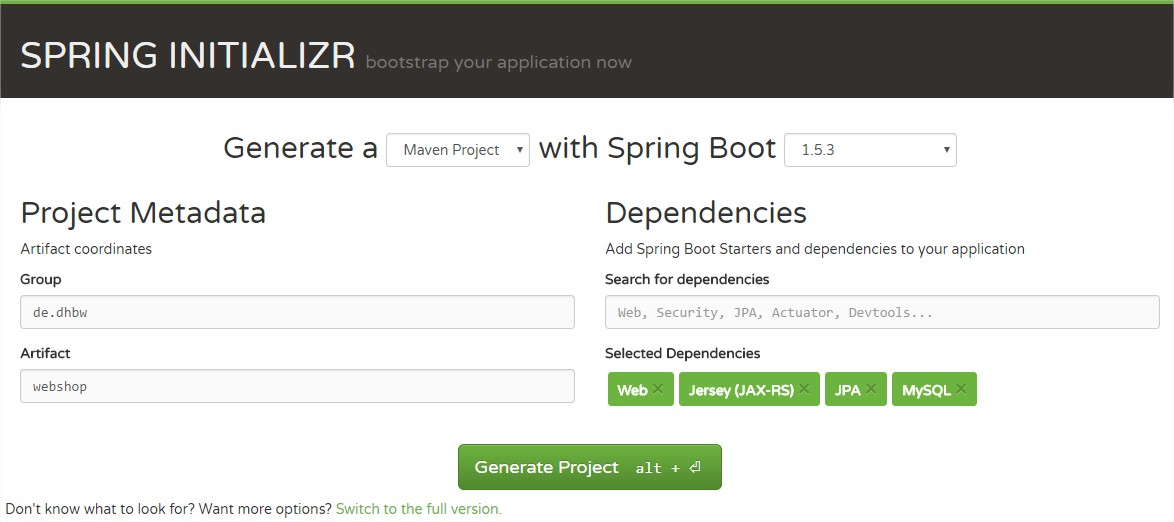
\includegraphics[width=\linewidth]{bilder/kap7/Spring-Initializr}
	\caption{Spring Inititalizr Weboberfläche}
	\label{fig:spring-initializr}
\end{figure}

\cref{fig:spring-initializr} zeigt die gewählte Konfiguration für das Grundprojekt. Links sind die Metadaten für das Deployment definiert und rechts die Abhängigkeiten. Diese sind initial:

\begin{itemize}
	\item \textit{Spring Web.} Wird benötigt um eine Webanwendung mit eingebettetem Tomcat-Server zu implementieren.
	\item \textit{Jersey.} Hierbei handelt es sich um die Referenzimplementierung von JAX-RS. JAX-RS ermöglicht es, anhand von Annotationen, herkömmliche Java-Klassen per REST verfügbar zu machen \cite{Oracle2015}.
	\item \textit{Spring Data JPA.} Stellt die Zugriffstechnologie der Java Persistence API (\acs{JPA}) zur Verfügung. Mit dieser Abhängigkeit können Datenzugriffsobjekte angelegt werden (sogenannte \acs{DAO}s, Data Access Objects), die alle notwendige Datenbankoperationen implementieren \cite{Webb2017}.
	\item \textit{Spring MySQL JDBC Driver.} Mit diesem Treiber kann die Spring Boot Anwendung automatisch eine Verbindung zur MySQL-Datenbank herstellen \cite{Webb2017}. Alle weitere Konfigurationen für diese Verbindung werden später in dieser Arbeit beschrieben.
\end{itemize}

Die Ordnerstruktur des generierten Projekts kann der \cref{fig:init-project} entnommen werden.
Es handelt sich hierbei um die übliche Struktur einer Java-Anwendung, mit einem \texttt{main} und einem \texttt{test} Verzeichnis.
Initial sind im \texttt{main} Verzeichnis nur zwei Dateien: die \texttt{WebshopApplication} Klasse und die \texttt{application.properties}.
Erstere enthält die Java \texttt{main}-Methode, welche die Anwendung lauffähig macht.
Dort werden auch automatisch alle notwendige Konfigurationen für Spring Boot gesetzt.
Die \texttt{application.properties} Datei ist zu diesem Zeitpunkt noch leer, aber sie wird später benutzt um unterschiedliche Aspekte der Anwendung (wie zum Beispiel Server-Port oder Verbindungsdaten zur Datenbank) auf einfache Art und Weise einzustellen.

Eine weitere wichtige Datei ist die \texttt{pom.xml} im Stammverzeichnis. Das Project Object Model oder \acs{POM} ist die grundlegende Arbeitseinheit von Maven.
Diese XML-Datei enthält Information über das Projekt, sowie Konfigurationsdetails, die von Maven verwendet werden um das Projekt zu bauen.
Einige dieser Konfigurationen betreffen beispielsweise Projekt-Abhängigkeiten, Plugins und Build-Profile \cite{Foundation2017}.

\begin{figure}[th!]
	\centering
	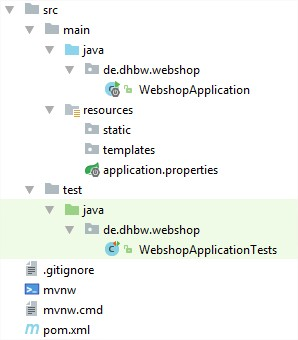
\includegraphics[width=0.5\linewidth]{bilder/kap7/init-project}
	\caption{Ordnerstruktur des generierten Projekts}
	\label{fig:init-project}
\end{figure}

\subsubsection{Angular 2 Anwendung}\label{angular_setup}
Auch hier wird ein Tool eingesetzt, um eine Basisanwendung zu generieren. Dabei handelt es sich um Angular CLI, ein Tool für die Initialisierung, Entwicklung und Wartung von Angular Anwendungen \cite{Arora2017}.

Angular CLI ist ein Open Source Projekt und wird anhand des Node Package Managers (\acs{NPM}) installiert.
Daraufhin stehen zahlreiche nützliche Befehle für die Kommandozeile zur Verfügung.
Für das Generieren einer Angular-Anwendung wird \texttt{ng init} ausgeführt. Der Befehl erstellt alle notwendige Ressourcen, sowie die komplette Konfiguration dazu.
Die statische Inhalte werden mit \texttt{ng build} gebaut.

Damit Spring Boot diese Inhalte verwenden kann, müssen sie jedoch im  \texttt{resources/static} Verzeichnis (siehe \cref{fig:init-project}) liegen.
Das kann durch einer Anpassung an der \texttt{angular-cli.json} Datei erreicht werden (Zeile 4 von \cref{lst:angular-cli}).
Des weiteren enthält diese Datei auch weitere wichtige Konfigurationen, wie der Ablageort von anderen Ressourcen wie Bildern oder benötigten Stylesheets.
An dieser Stelle werden demnach die \acs{CSS}-Dateien für das Bootstrap Framework referenziert, sowie ein eigenes Stylesheet für weitere Anpassungen.
Details zu Bootstrap und den Designentscheidungen werden später in dieser Arbeit beschrieben.
\\
\lstinputlisting[language=json,firstline=7,lastline=10,caption=Auszug der Datei angular-cli.json,label=lst:angular-cli]{listings/angular-cli.json}

\subsection{Backend-Klassen}
Wie bereits in \cref{outline_datamodel} beschrieben, gibt es für jede Entität in der Datenbank eine Klasse, die sie repräsentiert.
Um einzelne Datensätze aus der Datenbank zur Laufzeit in der Anwendung verwenden zu können, gibt es sogenannte \acs{DAO}-Klassen.
Diese gewährleisten den Zugriff auf die Datenbank und bieten außerdem Funktionen an, um bestimmte Datensätze über Abfragekriterien zu finden.
Von den \acs{DAO}-Klassen gelieferte Datensätze können als Instanzen der repräsentierenden Klasse weiterverwendet werden.
Für die Realisierung dieser Zugriffs-Klassen wurden Spring Data \acs{JPA} Repositories verwendet, die neben den grundlegenden \acs{CRUD}-Operationen eine Vielzahl an möglichen Abfragen ermöglichen.
\\
\lstinputlisting[language=Java,breaklines=true, firstline=15,caption=CategoryDao.java,label=lst:CategoryDao]{listings/CategoryDao.java}

\cref{lst:CategoryDao} zeigt eine solche \acs{DAO}-Klasse.
Zugriffs-Funktionen zu definieren kann auf unterschiedliche Art und Weise passieren. Zum einen ermöglichen diese Repositories es, Suchkriterien über den Namen der jeweiligen Funktion zu definieren.
So kann beispielsweise über eine Funktion \textit{findByName(String name)} der Datensatz mit dem der Funktion übergebenen Namen gefunden werden, wenn die Tabelle eine Spalte mit der Bezeichnung \enquote{Name} enthält.
Die Zuordnung auf die entsprechende Spalte in der Tabelle und die Suchfunktionalität müssen dabei nicht vom Entwickler implementiert werden.
Neben diesen semi-automatischen Funktionen können aber auch eigene Methoden definiert werden. Dafür kann über eine Annotation (@Query)eine \acs{SQL}-Query für die Abfrage an die Datenbank definiert werden.

\subsection{Objektrelationale Abbildung (\acs{ORM}) mit Hibernate}
Für die Zuordnung der Backend-Klassen zu den entsprechenden Tabellen in der Datenbank mit Hibernate stehen dem Entwickler eine Vielzahl von Annotationen zur Verfügung, von denen einige hier kurz beschrieben werden sollen.
Die Hibernate Annotation um eine Klasse als Entität zu markieren ist denkbar einfach. Sie wird direkt über der Klassendeklaration mit \textit{@Entity} gesetzt.
Darüber hinaus können auch der Tabellen-Name sowie die Namen der einzelnen Tabellenspalten über der Deklarationen der Klasse beziehungsweise des Attributs gesetzt werden.
Das ist allerdings nur für den Fall nötig, wenn diese Namen explizit vergeben werden sollen. Ansonsten werden sie von Hibernate gemäß dem Namen der Klasse in Kleinschriebung vergeben.
Wenn man aber die Zuordnung für eine bereits bestehende Datenbank machen möchte, sind diese expliziten Namen sehr hilfreich.
Ist eine entsprechende Tabelle beim Start der Anwendung nicht vorhanden, wird diese von Hibernate erzeugt.

Eine weitere wichtige Annotation betrifft die Primärschlüssel der Tabelle, die jeden Datensatz eindeutig identifizieren können. Mit \textit{@Id} kann dieses Attribut gekennzeichnet werden.
Empfehlenswert ist dabei die Verwendung eines künstlichen Schlüssels als Zahlenwert, der für jeden Eintrag hochgezählt wird.
Auch dafür bietet Hibernate eine komfortable Lösung, indem über \textit{@GeneratedValue} ein solcher generierter Wert definiert wird.
In Kombination mit einer automatischen Inkrementierung, die MySQL für numerische Werte bietet, kann also automatisch ein eindeutiger Zahlenwert für jeden neuen Eintrag in der Tabelle gesetzt werden.

Für die Beziehungen zu anderen Entitäten können entsprechend der Kardinalität folgende Annotationen verwendet werden:
\begin{itemize}
\item{@OneToOne.} 1:1
\item{@OneToMany.} 1:N
\item{@ManyToOne.} N:1
\item{@ManyToMany.} N:N
\end{itemize}

Über Parameter dieser Annotationen können neben der Ziel-Entität weitere Einstellungen (beispielsweise zum Cascading) gemacht werden, auf die hier nicht näher eingegangen werden soll.

\subsubsection{Vererbung von Klassen}
Eine Vererbungshierarchie von Klassen kann mit verschiedenen Strategien in der Datenbank abgebildet werden.
Hibernate bietet dafür vier grundlegende Varianten an \cite{Mihalcea2017}:
\paragraph{Mapped Superclass}$\;$ \\
In dieser einfachsten Form der Abbildung einer Vererbung wird für jede konkrete Ausprägung der vererbenden Klasse eine eigene Tabelle angelegt, die neben ihren eigenen auch alle Spalten der Eltern-Klasse enthält.
Die Vererbungshierarchie wird damit nicht explizit im Datenmodell ersichtlich.
\paragraph{Single table}$\;$ \\
Dabei werden alle erbenden Klassen in einer einzigen Tabelle in der Datenbank abgebildet. Dadurch enthält die Tabelle viele Spalten, da alle Attribute jeder Sub-Klasse enthalten sind.
Für einzelne Datensätze einer bestimmten erbenden Klasse werden nicht benötigte Spalten mit \enquote{null}-Werten belegt.
Um zu unterscheiden welche Datensätze zu welcher Sub-Klasse gehören, wird außerdem eine sogenannte \enquote{Discriminator Column} definiert.
Dieser Ansatz ist sehr performant, da für Abfragen immer nur eine Tabelle verwendet werden muss.
\paragraph{Table-per-subclass}$\;$ \\
Hier wird für die vererbende und jede erbende Klasse eine eigene Tabelle in der Datenbank erzeugt. Letzere enthalten dabei nur die Attribute, die sie zusätzlich zu den der Eltern-Klasse haben.
Die Zuordnung zur Eltern-Klasse wird über JOINS hergestellt, was die Performanz bei häufigen Abfragen negativ beeinflussen kann.
\paragraph{Table-per-concrete-class}$\;$ \\
In dieser letzten Variante wird wie bei Table-per-subclass für alle Entitäten eine Tabelle erzeugt. Diese enthalten jedoch jeweils alle eigenen und die Attribute der Eltern-Klasse.
Die Zuordnung wird über UNION-Operationen hergestellt, was ebenfalls zu Performance-Verlusten bei großen Klassen-Hierarchien führen kann.

Innerhalb des Webshops wurde für die Hierarchie bei Artikeln die \enquote{Single Table}-Strategie gewählt.
\cref{lst:inheritanceMapping} zeigt die Klassen-Definitionen mit den Annotationen für das \acs{ORM}.
\\
\lstinputlisting[language=Java, breaklines=true, caption=Vererbungshierarchie, label=lst:inheritanceMapping]{listings/Inheritance.java}

\subsection{REST-Schnittstellen}
Wie in \cref{spring-boot-init} bereits erwähnt, wurde für das Erstellen der REST-Services innerhalb der Spring Boot Anwendung Jersey als Implementierung der Java-Schnittstelle \acs{JAX-RS} benutzt.
Für die Darstellung der zu übertragenden Ressourcen verwendet JAX-RS standardmäßig die Implementierung von \acs{JAXB} (Java Architecture for XML Binding).
Der Vorteil daran ist, dass die Klassen mit der Annotation \texttt{@XmlRootElement} automatisch bei einem REST-Aufruf in die entsprechende XML- oder \acs{JSON}-Darstellung umgewandelt werden.
Die Unterstützung des JSON-Formates ist dadurch gewährleistet, dass JAXB die Jackson Bibliotheken benutzt.
Die Jackson Bibliothek bietet einen mächtigen Parser für die Konvertierung von Java-Objekten in JSON-Strings \cite{Oracle2015}.

Über Annotationen können normale Java-Klassen zu sogenannten Endpoints gemacht werden, die Anfragen über eine \acs{URI} entgegen nehmen und beantworten können.
Die wichtigsten sind \cite{Jersey2017a}:

\begin{itemize}
\item{@Path.} Legt die \acs{URI} für die Web-Services der Klasse oder einer Methode fest.
\item{@GET, @POST, @PUT, @DELETE, @HEAD.} Definiert die \acs{HTTP}-Methode für den Aufruf einer Service-Methode.
\item{@Consumes, @Produces.} Spezifiziert den \acs{MIME}-Typ, der von der Funktion konsumiert bzw. produziert werden kann.
\item{@*Param.} Wird verwendet, um Parameter bei der Anfrage auszulesen (z.B. \textit{@PathParam} für Paramter in der \acs{URI} der Anfrage).
\end{itemize}

Für die vorliegende Anwendung wurden die Endpoints thematisch separiert.
\cref{fig:endpoints} zeigt die definierten Endpoint-Klassen und ihre Implementierung.

\begin{figure}[th!]
	\centering
	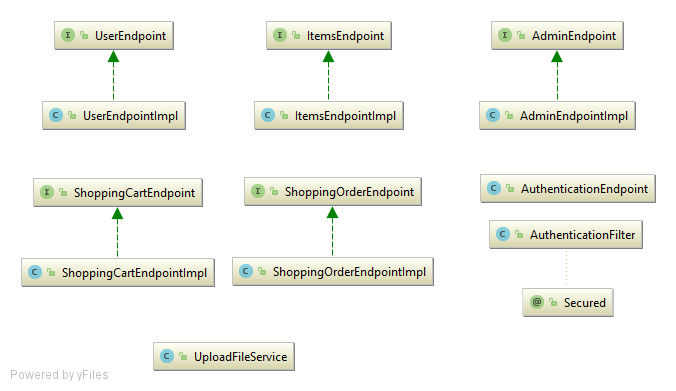
\includegraphics[width=0.75\linewidth]{bilder/kap7/api_diagram}
	\caption{REST-Endpoints}
	\label{fig:endpoints}
\end{figure}

Zusätzlich zu den Benutzer- und Administrator-Funktionalitäten wurden zwei weitere Endpoints für die Authentifizierung und den File-Upload erstellt.
\\
\lstinputlisting[language=Java,breaklines=true,caption=REST-Beispiel,label=lst:RESTexample]{listings/RESTexample.java}

\cref{lst:RESTexample} zeigt die Deklaration der Registrierungs-Funktion für Benutzer sowie deren Implementierung als Beispiel für die Endpoint-Funktionalitäten.

\subsection{Weitere Implementierungsdetails}
In diesem Abschnitt werden einzelne Details zur Implementierung vorgestellt.
Die dabei behandelten Themen resultierten aus der Notwendigkeit für eine bestimmte Funktionalität des Shops oder stellten ein Problem dar, für das eine Lösung gefunden werden musste.

\subsubsection{Passwort-Verschlüsselung}
Dass Passwörter nicht unverschlüsselt in einer Datenbank enthalten sein sollten, ist seit dem Diebstahl von persönlichen Nutzerdaten und -Zugängen bei großen Online-Anbietern nicht nur Fachleuten, sondern auch Laien bekannt.
Das Bundesamt für Sicherheit in der Informationstechnik \acs{BSI} gibt dafür offizielle Leitlinien heraus, in welcher Form das geschehen kann \cite{BSI2016}.
Auf die einzelnen Kryptographieverfahren und die Generierung solcher Schlüssel soll hier aber nicht weiter eingegeangen werden, sondern lediglich gezeigt werden, wie die Verschlüsselung in der Anwendung umgesetzt wurde.

Dabei wurde auf das bestehende Framework jBCrypt zurückgegriffen, eine Java-Implementierung des OpenBSD Blowfish Passwort-Hashing-Algorithmus \cite{jBCrypt2015}.
Dieser benutzt eine 64-Bit Block-Cipher, um einen Hash des Passworts zu generieren, der dann in der Datenbank gespeichert werden kann \cite{Provos}.
Beim Registrieren eines Nutzers wird sein Passwort über das Framework zu einem Hash-Wert verarbeitet und gespeichert.
Wenn ein User sich am System anmeldet, wird das im Klartext eingegebene Passwort wiederum mit dem gespeicherten Hash-Wert verglichen, was erneut vom Framework bewerkstelligt wird.

\subsubsection{Token-Authentifizierung}\label{token}
Um zu vermeiden, dass sich ein Benutzer für jede Anfrage an den Server immer wieder anmelden muss, wurde auf die Verwendung einer Token-Authentifizierung zurückgegriffen.

\acs{JSON} Web Token (\acs{JWT}) ist ein offener Standard für die sichere Übermittlung von \acs{JSON}-Objekten zwischen zwei Partnern und wird häufig für die Authentifizierung bei Web-Anwendungen verwendet.
Durch eine digitale Signierung mit einem Verschlüsselungs-Algorithmus sind die Tokens fälschungssicher. Außerdem können im Token selbst zusätzliche Informationen gehalten werden.
Diese können beispielsweise verwendet werden, um den Benutzer zu identifizieren, wodurch bei einer erneuten Anfrage nicht zuerst wieder eine Datenbank-Abfrage nötig wird \cite{Auth02016}.

Für den Webshop wurde \acs{JWT} integriert, indem beim Login ein Token erstellt und übermittelt wird. Für erneute Anfragen wird dieses mitgeschickt. Als zusätzliche Information enthält es die User-Id und die Rolle des Benutzers (User oder Admin).
Bei sämtlichen REST-Endpoint-Methoden, die eine Anmeldung erfordern, wird das Token und für die Admin-Funktionalitäten zusätzlich die Rolle überprüft.

\subsubsection{File Upload}
Für das Hochladen und Speichern von Dateien oder Bildern durch Benutzer gibt es in Web-Anwendungen verschiedene Realisierungsmöglichkeiten.
Wie bei allen Eingaben, die von Usern gemacht werden, muss dabei auch auf die Sicherheit geachtet werden, da durch solche Operationen Schaden an der Anwendung oder der Datenbank angerichtet werden können.
Da in der vorliegenden Anwendungen der Upload von Bild-Daten nur von Administratoren durchgeführt werden kann, ist dieser Aspekt aber vernachlässigbar.

Um Bilder für Artikel persistent zu speichern und auch bei einer möglichen Neu-Installation der Anwendung verfügbar zu haben, wurde eine Lösung gewählt, die die Bilder mit den Artikeldaten in der Datenbank speichert.
Der Datentyp \acs{Blob} (Binary Large Object) ermöglicht das Speichern eines simplen binären Byte-Arrays, das beim Upload direkt als Stream geschrieben werden kann.
Eine dafür erstellte REST-Endpoint-Funktion liefert dann für einen Artikel das entsprechende Bild zurück, das im Frontend angezeigt werden kann.

\subsection{Frontend}
Dieser Abschnitt behandelt die Details zur Implementierung der Angular 2 Anwendung. Die Gliederung ist so aufgebaut, dass einige der in \cref{angular_arch} beschriebenen Architekturelemente mit der konkreten Umsetzung im Rahmen dieses Projekts vertieft werden.

\subsubsection{Module}
Es ist weitestgehend den Entwicklern überlassen, welche Funktionalitäten in welcher Form zu Angular-Modulen gekapselt werden. Prinzipiell wäre es auch möglich, eine Anwendung ganz ohne Module zu erstellen (abgesehen vom bereits erwähnten, obligatorischen Root-Modul). Im Webshop wurden jedoch der Übersichtlichkeit halber zwei Module definiert: ein Shop- und ein Admin-Modul. Somit ist die Trennung zwischen diesen Bereichen auch in der Implementierung gegeben.

Beide Module enthalten eine Modul-Klasse, eine Basiskomponente mit Template, sowie ein Routing-Modul, das importiert wird. Die Aufgabe der Routing-Module ist es, beim Aufruf einer bestimmten URL der Webseite eine dazu zugewiesene Komponente in einen Platzhalter des \acs{DOM}s zu laden.
\\
\lstinputlisting[language=JavaScript,breaklines=true,caption=Routing-Module,label=lst:routing]{listings/routing.ts}

\cref{lst:routing} zeigt einige der Routen des Shop-Moduls. Wie in Zeile 2 zu sehen ist, sind alle URLs des Webshops unter dem Pfad \enquote{shop} definiert, der die Hauptkomponente des Moduls repräsentiert. Im Template dieser Komponente ist der bereits erwähnte Platzhalter für die Kind-Komponenten enthalten. Die Eigenschaft \texttt{canActivate} der Pfade sagt aus, dass diese URL geschützt ist und ausschließlich angemeldete Benutzer darauf zugreifen können. Dafür wird eine Funktion ausgeführt die überprüft, ob bereits ein Benutzer angemeldet ist und im negativen Fall eine Weiterleitung zur Login-Komponente tätigt.

\subsubsection{Komponenten}
Die Anwendung ist so aufgebaut, dass für den Inhalt jeder Seite eine Komponente existiert. Diese kann wiederum aus weiteren Komponenten bestehen, die in das Template eingebunden werden. Ein Beispiel dafür ist die Produktauflistung zu jedem Kategorie-Reiter. Alle Seiten dieser Art sehen wie auf \cref{fig:items_list} aus. Die roten Markierungen identifizieren die zwei Kind-Komponenten, die eingebunden sind.

\begin{figure}[th!]
	\centering
	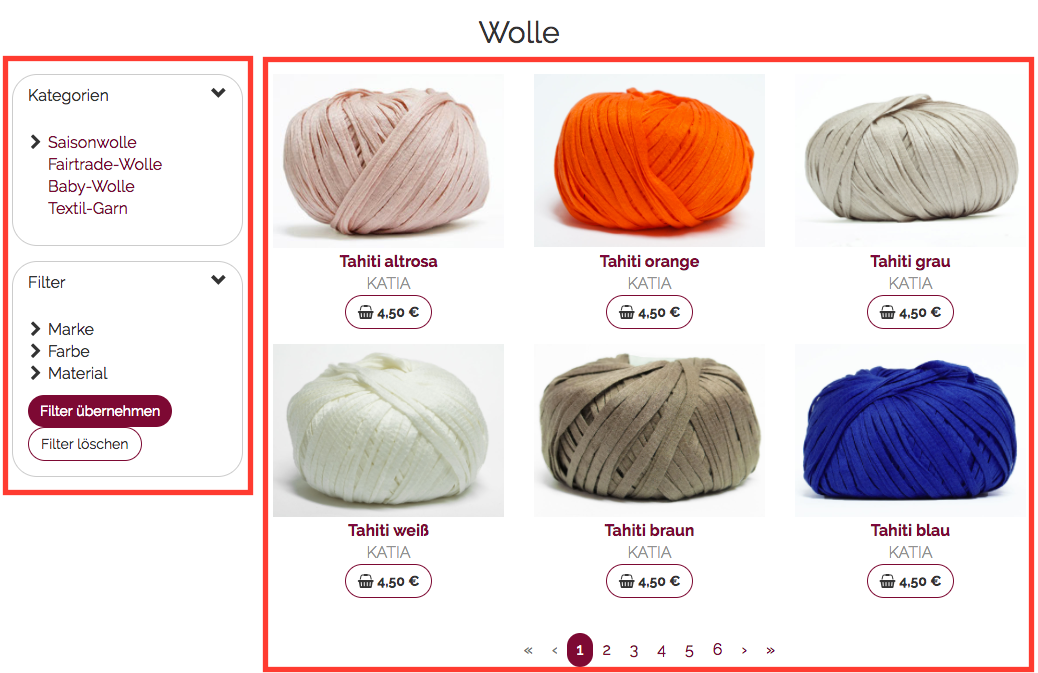
\includegraphics[width=0.8\linewidth]{bilder/kap7/items}
	\caption{Inhalt der Seite für die Kategorie Wolle}
	\label{fig:items_list}
\end{figure}

Wie diese Seite realisiert wurde ist in \cref{lst:item-template} veranschaulicht. Die Einbindung der Unterkomponenten erfolgt jeweils in Zeilen 4 und 8. Die Attribute in orangefarbener Schrift sind sogenannte \textit{Inputs} der Komponente, eine Form des Data-Binding, die in \cref{angular_arch} bereits beschrieben wurde.
\\
\lstinputlisting[language=HTML5,breaklines=true,caption=Template für die Produklisten-Komponente,label=lst:item-template]{listings/items-template.html}

\subsubsection{Services}
Alle Methoden zum Aufruf der \acs{REST}-Schnittstellen sind in mehrere Services gekapselt. In der Angular Anwendung gibt es einen Service für jede auf \cref{fig:endpoints} dargestellte Schnittstelle, sozusagen als Gegenstück davon. \cref{lst:service} zeigt beispielsweise die Methode zum Aufruf des Warenkorbes eines Benutzers.
\\
\lstinputlisting[language=JavaScript,breaklines=true,caption=Methode für den Aufruf des Warenkorbes,label=lst:service]{listings/service.ts}

In den Zeilen 3 und 4 von \cref{lst:service} wird der Authentifizierungs-Header für die HTTP-Anfrage vorbereitet. Der Header besteht aus einem JWT-Token (siehe \cref{token}), der beim Login in der Anwendung gespeichert wird. Die Anfrage selbst beginnt in Zeile 6, mit dem Aufruf der GET-Methode. Diese und alle weitere HTTP-Methoden sind in Angular durch ein eigenes Modul gewährleistet. Wie man sieht erhält die Methode als Parameter die URL zum gewünschten REST-Endpoint und die Header. Der Rückgabewert des asynchronen Aufrufs ist ein sogenanntes \textit{Observable}-Objekt der RxJS-Bibliothek. Diese Bibliothek implementiert in JavaScript das Observer-Pattern, ein Verhaltensmuster das zur Weitergabe von Änderungen an einem Objekt an andere beobachtenden Objekte dient \cite{Angular.io2017b}.

\newpage
Zwei der wichtigsten Methoden eines RxJS Observable-Objekts sind in \cref{lst:service} zu sehen. Zum einen die \texttt{map()}-Funktion in Zeile 7 und zum anderen \texttt{subscribe()} in der darunterliegenden Zeile. Erstere dient zur Transformation der empfangenen Daten, in diesem Fall das Parsen von den Daten zu einem JSON-Objekt. Die \texttt{subscribe()}-Funktion ermöglicht es, das Observable-Objekt im Hinblick auf jegliche Änderungen zu beobachten (im dargestellten Beispiel die Daten aus dem asynchronen Aufruf und eventuelle Fehlermeldungen). Sobald eine Änderung erkannt bzw. eine Antwort vom Server erhalten wird, können beliebige Aktionen mit den Daten durchgeführt werden.

Ein weiterer Anwendungsfall des Observer-Patterns in Angular-Anwendungen sind die Interaktionen zwischen Komponenten, die nicht direkt miteinander verwandt sind (keine Eltern-Kind-Beziehung). Auch davon ist in \cref{lst:service} ein Beispiel zu sehen. Das \texttt{shoppingCartUpdate}-Objekt in Zeile 12 ist im Service als ein sogenannter \textit{EventEmitter} deklariert. Andere Komponenten und Services der Anwendung können mit \texttt{subscribe()} dieses Objekt beobachten. Wird wie in Zeile 12 die Methode \texttt{next()} mit einem neuen Wert aufgerufen, bekommen alle Beobachter die Änderung mit.

\subsubsection{Styling}

In \cref{angular_setup} wurde bereits erwähnt, dass im Frontend das Bootstrap Framework für das Design der Oberfläche verwendet wird. Grund dafür ist, dass Bootrap besonders für die Entwicklung von Anwendungen mit Responsive Design konzipiert ist. Traditionell wurde die Aufteilung der Elemente auf einer Webseite mit Tabellen gemacht, die jedoch schwer zu skalieren sind. Die Lösung von Bootstrap ist das sogenannte \textit{Grid System}. Hierbei ist die Oberfläche in Zeilen mit jeweils zwölf virtuellen Spalten mit skalierbarer Breite aufgeteilt. \cref{lst:item-template} auf Seite \pageref{lst:item-template} zeigt, wie das Grid System eingesetzt werden kann. Mit der CSS-Klasse \texttt{col} können beliebige Spalten-Kombinationen für unterschiedliche Display-Größen erstellt werden.
